\documentclass{book}

\usepackage[portuguese]{babel}
\usepackage{geometry}
\usepackage{float}
\usepackage{graphicx}
\usepackage{amsthm}

\graphicspath{ {./figures} }

\theoremstyle{definition}
\newtheorem{definition}{Definição}

\newgeometry{vmargin={20mm}, hmargin={22mm,22mm}}

\title{Apontamentos de BD}
\author{João Aragonez}
\date{}




\begin{document}

\maketitle
\tableofcontents


\chapter{Conceitos Iniciais}

\section{Sistemas de informação}
\begin{definition}[Sistemas de Informação]
    Consiste na área que estuda as atividades de pendor estratégico, operacional e de gestão subjacentes à recolha, processamento, armazenamento, distribuição e uso de informação e de tecnologias associadas, tanto pela sociedade como por organizações. \\
    \indent Também é comum definir SI como a interação entre tecnologia e processos de negócio, mais concretamente, a gestão de 3 componentes fundamentais: \textbf{dados, tecnologia e pessoas}.
\end{definition}
Entre outros, menciona-se os seguintes tipos de sistemas de informação:
\begin{itemize}
    \itemsep0cm
    \item[--] \textit{ERP} (\textit{Enterprise Resource Planning});
    \item[--] SIG (Sistemas de Informação Geográfica);
    \item[--] Sistemas de \textit{office automation};
    \item[--] Sistemas de \textit{Business Intelligence};
    \item[--] Sistemas Especialistas;
    \item[--] \textit{WWW} (\textit{World Wide Web}).   
\end{itemize}

\section{Sistemas de Gestão de Bases de Dados (SGBD)}

\begin{definition}[Base de Dados]
    Consiste em nada mais que conjuntos de dados interligados.
\end{definition}

\begin{definition}[Sistema de Gestão de Bases de Dados]
    Consiste numa ferramenta de software desenhada para a manutenção e gestão de bases de dados
\end{definition}

Dado que os sistemas operativos atuais se encontram munidos de um sistema de ficheiros, perfeitamente capazes de lidar com o armazenamento de informação, surge a seguinte questão: \textit{porquê usar um SGBD?} A verdade é que os sistemas de informação apresentam necessidades comuns que não são cobertas por sistemas de ficheiros. Assim, os SGBD têm por objetivo realizar:

\begin{itemize}
    \itemsep0cm
    \item[--] Controlo de redundância;
    \item[--] Segurança e controlo de acessos, dada a heterogeneidade de utilizadores e de dados;
    \item[--] Persistência de dados;
    \item[--] Oferecer múltiplas interfaces para diferentes tipos de utilizadores;
    \item[--] Representar relações complexas;
    \item[--] Assegurar constrangimentos de integridade sobre os dados;
    \item[--] Realizar controlo de concorrência, por forma a manter os dados consistentes;
    \item[--] Permitir que uma grande quantidade de iterrogações (\textit{queries}) possam ser feitas sobre os dados sem necessidade de programação adicional;   
    \item[--] Garantir tolerância a faltas (e.g., realizando \textit{backups}). 
\end{itemize}

\subsection{Vantagens dos SGBD's}
\vspace{0.25cm}

\begin{itemize}
    \itemsep0cm
    \item[--]\textbf{Independência dos dados}: encapsulando o modo real de representação e armazenamento dos dados, os SGBD's disponibilizam uma visão abstrata dos dados.
    \item[--]\textbf{Acesso Eficiente aos Dados}: os SGBD incorporam técnicas para armazenamento e recolha eficiente dos dados;
    \item[--]\textbf{Integridade dos dados e segurança}: os SGBD garantem a aplicação de restrições de integridade no acesso e manipulação de dados;
    \item[--]\textbf{Capacidade de administração dos dados}: é possível mudar a representação dos dados por forma a minimizar a redundância e melhorar o armazenamento de forma totalmente transparente ao utilizador;
    \item[--]\textbf{Acesso Concorrente e Recuperação de Falhas}: existe suporte à concorrência no acesso aos dados, garantido um efeito semelhante a um acesso sequencial;
    \item[--]\textbf{Redução do tempo de desenvolvimento de aplicações}: disponibiliza uma interface de alto nível para os dados e funções de acesso comuns, sendo para além disso uma componente da aplicação que não necessita de ser verificada.  
\end{itemize}

\subsection{Desvantagens dos SGBD's}

\begin{itemize}
    \itemsep0cm
    \item[--]\textbf{Overhead demasiado elevado}: requer investimento em hardware, software e formação no uso destes sistemas;
    \item[--]\textbf{Tratamento demasiado geral}: Dependendo da aplicação, os mecanismos de segurança, controlo de concorrência, integridade e de recuperação de faltas podem não ser suficientes;
    \item[--]\textbf{Desadequados a sistemas com requisitos de tempo-real};
    \item[--]\textbf{Desadequados a bases de dados simples/imutáveis ou sem concorrência de acessos};
    \item[--]\textbf{Desadequados a certos tipos de dados, como texto}.   
\end{itemize}

\section{Modelos e Níveis de Abstração nos SI}

Num SGBD, os dados podem ser descritos segundo diversos modelos, que correspondem a diferentes níveis de abstração acerca da sua representação/armezenamento:
\begin{itemize}
    \itemsep0cm
    \item[--]\textbf{Modelo Conceptual} (ou esquema externo), que descreve como os utilizadores vêm os dados. Permite particulizar o acesso aos dados através de \textbf{Vistas} - conjuntos de registos visíveis para grupos específicos de utilizadores e apenas computados quando necessário (i.e., não são explicitamente armazenados). Este nível permite \textbf{independência dos dados lógicos}, pois alterações ao esquema lógico requerem unicamente redefinição de vistas, pelo que o utilizador não se dará conta de eventuais extensões e modificações das estruturas de dados.
    \item[--]\textbf{Modelo Lógico} (ou esquema conceptual), que corresponde à estrutura lógica dos dados (e.g., relações existentes no modelo relacional). Este nível permite \textbf{independência dos dados físicos}, pois a organização física nada influi sobre o esquema lógico dos dados.
    \item[--]\textbf{Modelo Interno} (ou esquema físico), que especifica os detalhes de armazenamento das relações (e.g., definição de tipos de ficheiros a utilizar e de índices). 
\end{itemize}
\begin{figure}[H]
    \centering
    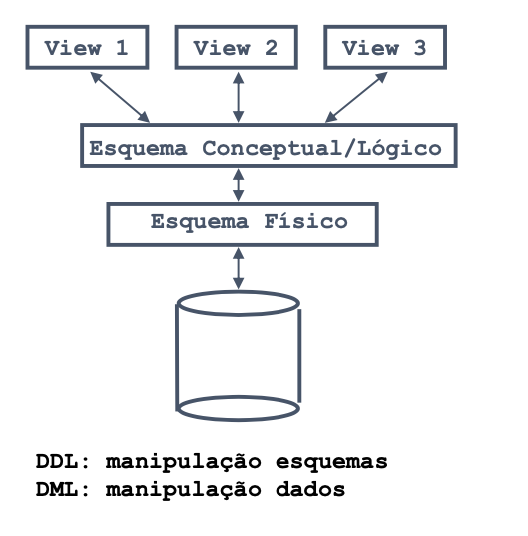
\includegraphics[scale = 0.6]{cap1/modelo_ansi.png}
    \caption{Modelo \textit{ANSI/SPARC}}
\end{figure}

\section{Modelos de Dados}

\begin{definition}[Modelo de Dados]
    Coleção de conceitos para descrever dados, relacionamentos, semântica de dados e restrições.
\end{definition}
\begin{definition}[Esquema]
    Descrição de uma coleção específica de dados à luz de um dado modelo de dados (i.e., o resultado da aplicação de um modelo de dados um conjunto de dados específico).
\end{definition}

Entre outros modelos de dados, destacam-se o \textbf{Modelo Relacional}, o \textbf{Modelo Entidade-Associação}, o \textbf{Modelo Baseado em Objetos}, \textbf{Modelos de Dados Semi-Estruturados} (como \textit{XML/JSON}), ou os \textbf{Modelos em Rede e Hierárquicos} (não usados atualmente).\\
\indent Contudo, o modelo de dados mais amplamente difuso nos SGDB é o \textbf{modelo relacional}, cujos conceitos fundamentais são a \textbf{relação} (i.e., um tuplo de atributos) e o \textbf{esquema}, que corresponde à especificação do nome da relação e do nome e tipo dos seus atributos. \\
\indent Numa fase mais inicial do desenvolvimento de bases de dados, podem-se usar \textbf{Modelos Semânticos de Dados}, passíveis de serem diretamente traduzidos para o modelo relacional. O exemplo mais paradigmático destes modelos é o \textbf{Modelo Entidade-Associação}.

\section{Arquitetura dos SGBD}

As arquiteturas dos SGBD procuram, por um lado, maximizar a \textbf{eficiência e escalabilidade}, mais concretamente, acelerando as interrogações sobre os dados. A figura abaixo exibe as fases que compõem o processamento de uma \textit{query}: \textbf{análise e tradução}, \textbf{otimização} e  \textbf{avaliação}.

\begin{figure}[H]
    \centering
    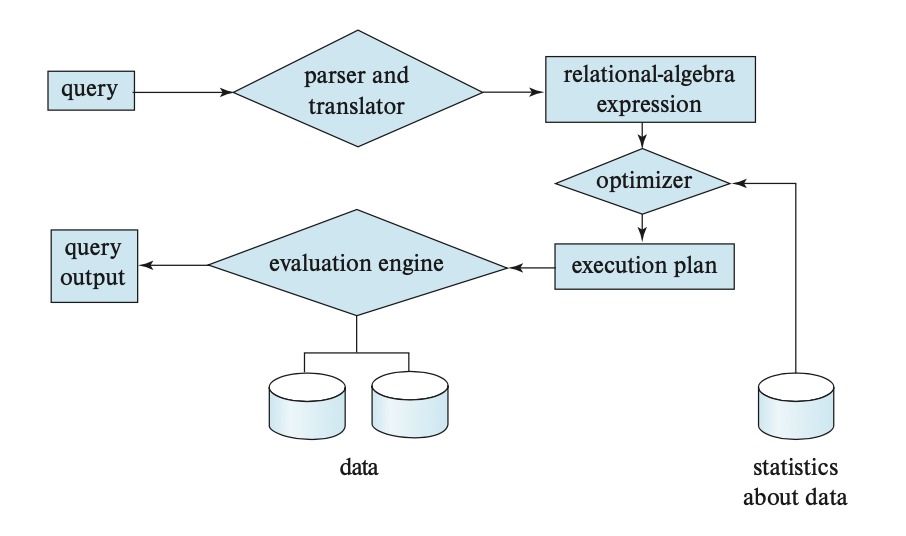
\includegraphics[scale = 0.5]{cap1/arquitetura.png}
    \caption{Processamento de uma \textit{query}}
\end{figure}

Por outro lado, procuram maximizar a \textbf{concorrência e a robustez}, existindo um \textbf{gestor de transações} para lidar com questões de concorrência, bem como um \textbf{gestor de recuperação} e um \textbf{gestor de \textit{locks}}.

\begin{figure}[H]
    \centering
    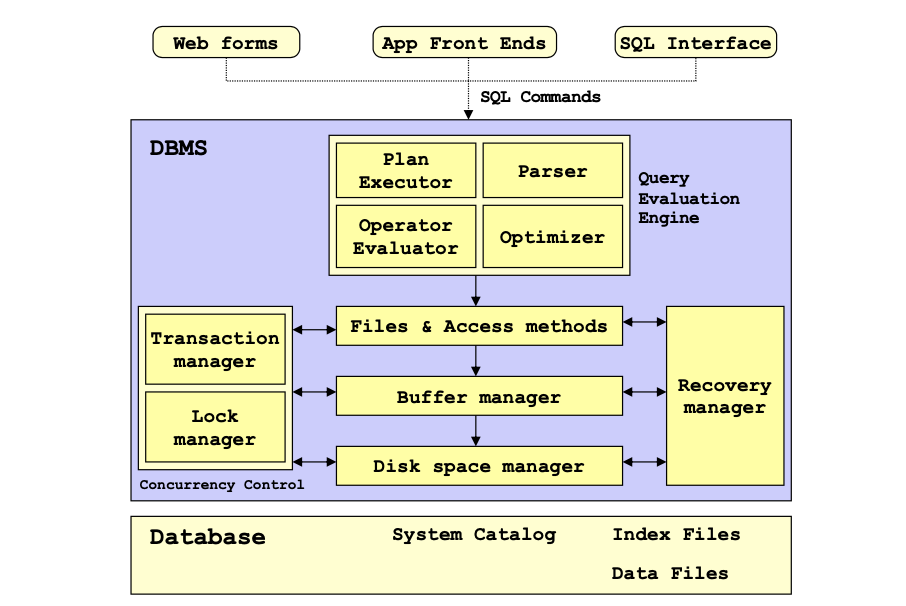
\includegraphics[scale = 0.75]{cap1/arquitetura_geral.png}
    \caption{Arquitetura de um SGBD}
\end{figure}

\section{Conceção de Bases de Dados}

O processo de conceção de um base de dados incide inicialmente no \textbf{desenho lógico}, i.e., sobre o \textbf{esquema} a adotar. Para este decisão contribuem fatores associados ao \textbf{Negócio} (como determinar quais os atributos mais relevantes para o domínio em questão), bem como fatores de \textbf{Engenharia}, como definição de esquemas e distribuição dos atributos por estes.

\section{Utilizadores de Bases de Dados}

\begin{itemize}
    \item[--] \textbf{Implementadores de Bases de Dados;}
    \item[--] \textbf{Utilizadores das aplicações;} 
    \item[--]\textbf{Programadores de aplicações} ao definirem o modelo lógico do sistema de informação;
    \item[--] \textbf{DBA} (\textit{Database Administrators}), que concebem e mantêm a base de dados, em termos de desenho físico e lógico, segurança e configuração dos mecanismos de disponibilidade e recuperação. 
\end{itemize}





\end{document}